\documentclass{article}
\usepackage[utf8]{inputenc}
\usepackage[a4paper, total={6in, 8in}]{geometry}
\usepackage{graphicx}
\usepackage{amsmath}
\usepackage{enumitem}

\title{Econ 20000-Problem Set 5}
\author{Dr. Fulya Ersoy}
\date{}
\begin{document}
\maketitle
\begin{enumerate}
\item  Suppose a consumer's marginal willingness-to-pay (inverse Marshallian demand curve) is given by $p_1 = 10-4x_1$.
\begin{enumerate}[label=(\alph*)]
\item Calculate the change in consumer surplus for this consumer when the price of good 1 decreases from $p_1= 4$ to $p_1 = 2$ using the integral version of the formula.
\item[] $x_1(p_1)=\frac{10-p_1}{4}\Rightarrow\Delta CS=-\int^{p_1^f}_{p_1^o}x_1(p_1)dp_1=-\int^2_4\frac{10-p_1}{4}dp_1=-\frac{1}{4}(10p_1-\frac{1}{2}p_1^2 \Big|^2_4)$
\item[] $\Rightarrow-\frac{1}{4}((10(2)-\frac{1}{2}(2)^2)-(10(4)-\frac{1}{2}(4)^2   ))=-\frac{1}{4}((20-2)-(40-8))=-\frac{1}{4}(18-32)=3.5$
\item Sketch a graph to illustrate the change in consumer surplus described here.
\item[]
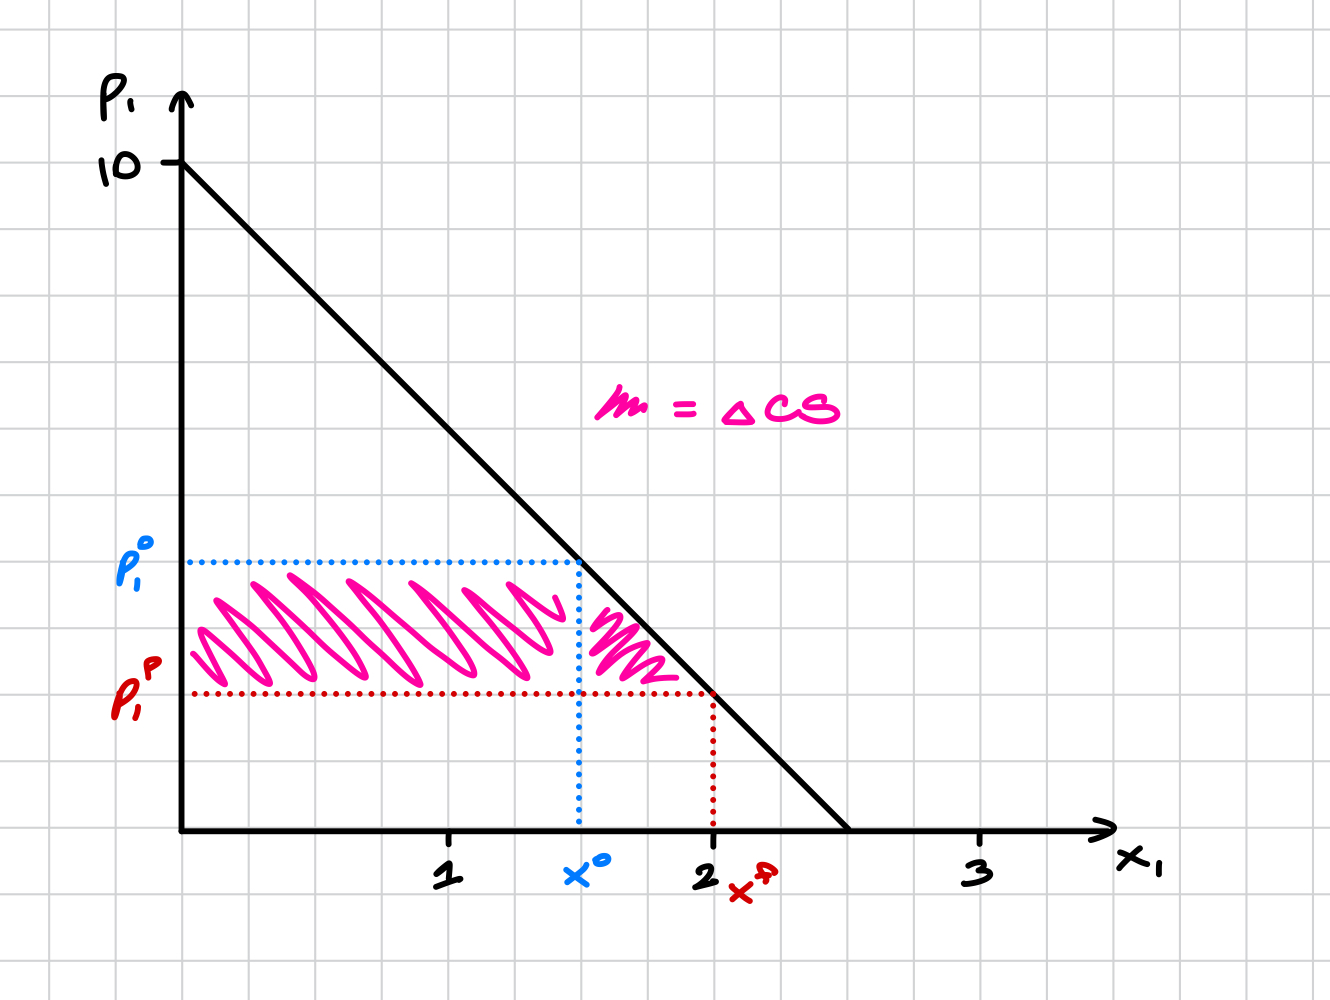
\includegraphics[width=8cm]{ECON 20000 PSet 5 Image 1.jpeg}
\item Using the graph, verify the answer you find in part (a) is indeed the change in consumer surplus. 
\item[] As shown in the graph, the area is given by $(4-2)\cdot(1.5)+\frac{1}{2}((4-2)\cdot(2-1.5))=3.5$
\end{enumerate}
\item Suppose that a consumer's utility function is given by $U(x,y)=ln(x)+y$. Suppose that price of good x increases from $p_x^o$ to $p_x^f$. Prove that compensating variation (CV), equivalent variation (EV) and change in consumer's surplus are all equal to each other. Why is this the case? Hint: Calculate Hicksian and Marshallian Demand functions for good x and use the integral version of the formulas. 
\item[] Marshallian Demand: Budget constraint of $p_xx+y=m$ yields utility of $\max_x=lnx+m-p_xx$. FOC $=\frac{1}{x}-p_x=0\Rightarrow x_M(p_x)=\frac{1}{p_x}$. This represents quasi-linear utility, independent of income. Associated $y_M=m-p_xx_M=m-p_x\cdot\frac{1}{p_x}=m-1$. Thus, $v(p_x,m)=-lnp_x+m-1$.
\item[] Hicksian Demand: Expenditure function is found by minimizing $e=p_xx+y$ s.t. $lnx+y=u$. Thus, $e(p_x,\bar u)=p_xx+u-lnx$. FOC $=p_x-\frac{1}{x}\Rightarrow x_H(p_x,u)=\frac{1}{p_x}$. Also quasi-linear, equal to Marshallian Demand. Plugging back in: $e(p_x, u)=p_x\cdot\frac{1}{p_x}+ u-ln(\frac{1}{p_x})=1+ u+lnp_x$.
\item[] $CV=e(p_x^f,u^o)-e(p_x^o,u^o)=(1+u^o+lnp_x^f)-(1+u^o+lnp_x^o)=ln(\frac{p_x^f}{p_x^o})$.
\item[] $EV=e(p_x^0,u^o)-e(p_x^o,u^f)=(1+u^0+lnp_x^o)-(1+u^f+lnp_x^o)=u^o-u^f$.
\item[] Substituting Marshallian indirect utility found above: $u^o=-lnp_x^0+m-1$, $u^f=-lnp_x^f+m-1$. Thus, $u^o-u^f=(-lnp_x^o+m-1)-(-lnp_x^f+m-1)=ln(\frac{p_x^f}{p_x^o})$.
\item[] $\Delta CS=\int^{p_x^f}_{p_x^o}x_M(p_x)dp_x=\int^{p_x^f}_{p_x^o}\frac{1}{p_x}dp_x=ln(\frac{p_x^f}{p_x^o})$.
Therefore, $\Delta CS=EV=CV=ln(\frac{p_x^f}{p_x^o})$.
\item Jessica has \$12 to spend on fruit and salads. Her utility function is given by $u(F, S)=F^{0.5}S^{0.5}.$ $p_F^o=\$2$ per lb and $p_S=\$1$ per lb. Suppose the price of fruits increased to $p_F^f=\$3$ per lb.
\begin{enumerate}[label=(\alph*)]
\item Solve the UMP and find Marshallian Demand Function for Fruits and Salads for generic $p_F, p_S, m$.
\item[] UMP: $\max_{x,y} u(F,S)=F^{\frac{1}{2}}S^{\frac{1}{2}}$ s.t. $p_FF+p_SS=m$. Cobb-Douglas: $F^*=\frac{m}{2p_F}$, $S^*=\frac{m}{2p_S}$. 
\item Calculate the indirect utility function for generic $p_F, p_S, m$.
\item[] Substitute demand functions into $u$: $u=\sqrt{FS}=\sqrt{\frac{m}{2p_F}\cdot\frac{m}{2p_S}}=\frac{m}{2\sqrt{p_Fp_S}}=v(p_F,p_S,m)$.
\item Find the expenditure minimization function for generic $p_F, p_S, \bar{u}$ using duality.
\item[] EMP: $v(p_F,p_S,e(p_F,p_S,\bar u))=\bar u=e(p_F,p_S,v(p_F,p_S,m))=m$, by duality.
\item[] Therefore, $\Rightarrow\frac{m}{2\sqrt{p_Fp_S}}=\bar u\Rightarrow m=2\bar u\sqrt{p_Fp_S}=e(p_F,p_S,\bar u)$.
\item Calculate the Compensating Variation.
\item[] $CV=e(p_F^f,p_S,u^o)-m=2u^o\sqrt{p_F^fp_S}-m=(2\cdot\sqrt{\frac{12}{2\cdot2}\cdot\frac{12}{2\cdot1}}\cdot\sqrt{3\cdot1})-12=2\cdot3\sqrt{2}\cdot\sqrt{3}-12=6\sqrt{6}-12\approx2.697$.
\item Calculate the Equivalent Variation.
\item[] $EV=m-e(p_F^o,p_S,u^f)=12-2u^f\sqrt{p_F^op_S}=12-(2\cdot\sqrt{\frac{12}{2\cdot 3}\cdot\frac{12}{2\cdot 1}}\cdot \sqrt{2\cdot 1})=12-2\cdot 2\sqrt{3}\cdot \sqrt{2}=12-4\sqrt{6}\approx 2.202$.
\item Calculate the Change in Consumer Surplus.
\item[] $\Delta CS=\int^{p_F^f}_{p_F^o}F(p_F)dp_F=\int^3_2\frac{m}{2p_F}dp_F=\frac{m}{2}\int^3_2\frac{1}{p_F}dp_F=\frac{m}{2}ln(\frac{3}{2})=6ln(\frac{3}{2})\approx2.433$.
\item What is the relationship between the three? Based on this relationship, what can you infer about fruits for Jessica? Are they a normal good or inferior good?
\item[] $CV>\Delta CS>EV$. Thus, fruits are a normal good. A decrease in purchasing power (increase in price) reduces demand for the good, so the compensated demand associated with the lower utility level lies below the resulting one with the higher utility level. Further, the income needed to restore old utility ($CV$) is largest, the income needed to anticipate new utility ($EV$) is smallest, and Marshallian measure ($\Delta CS$) lies in between.
\end{enumerate}
\end{enumerate}
\end{document}